% =====================================================================
%  MolGraph-AE — Project Report
%  Indian Institute of Science Education and Research (IISER), Pune
%  Supervisor: Dr. Arnab Mukherjee
%
%  COMPILE:  pdflatex main.tex   (run twice for cross-references)
%  Requires: graphicx, tikz, booktabs, amsmath, hyperref, geometry
%
%  Figure paths are relative to the repository root (one level up).
% =====================================================================
\documentclass[11pt,a4paper]{article}

\usepackage[margin=2.4cm]{geometry}
\usepackage{graphicx}
\usepackage{amsmath,amssymb}
\usepackage{booktabs}
\usepackage{tikz}
\usepackage{xcolor}
\usepackage{caption}
\usepackage{subcaption}
\usepackage[hidelinks]{hyperref}
\usepackage{float}

\usetikzlibrary{arrows.meta,positioning,fit,backgrounds,shapes.geometric,calc}

% Explicit paths only. NOTE: trajectory_pre_/loss_curve.png and
% temporal_dynamics/loss_curve.png share a filename, so a graphicspath search
% list would silently resolve the Stage-3 figure to the Stage-2 curve.
\graphicspath{{../}}

% ---- TikZ styles -----------------------------------------------------
\tikzset{
  blk/.style   ={rectangle, rounded corners=2pt, draw=black!70, fill=blue!6,
                 minimum height=8mm, minimum width=24mm, align=center, font=\small},
  dat/.style   ={rectangle, draw=black!55, fill=gray!10, minimum height=8mm,
                 minimum width=22mm, align=center, font=\small},
  loss/.style  ={rectangle, rounded corners=2pt, draw=red!60, fill=red!7,
                 minimum height=8mm, align=center, font=\small},
  frozen/.style={rectangle, rounded corners=2pt, draw=black!70, fill=green!8,
                 minimum height=8mm, minimum width=24mm, align=center, font=\small},
  ar/.style    ={-{Stealth[length=2.2mm]}, thick, draw=black!70},
}

\newcommand{\phipsi}{$(\phi,\psi)$}

% =====================================================================
\begin{document}

\begin{titlepage}
\centering
\vspace*{1.4cm}

{\LARGE\bfseries MolGraph-AE\par}
\vspace{0.5cm}
{\large A Three-Stage Deep Learning Pipeline for\\[2pt]
Generative Modelling of Dipeptide Conformational Dynamics\par}

\vspace{1.4cm}
\rule{\textwidth}{0.5pt}
\vspace{0.4cm}

{\large
Graph Autoencoding, Distribution Matching, and\\
Equivariant Flow-Matching Trajectory Propagation\par}

\vspace{0.4cm}
\rule{\textwidth}{0.5pt}

\vfill

{\large\bfseries Research Internship Report\par}
\vspace{0.8cm}

{\large Submitted to\par}
\vspace{0.3cm}
{\large\bfseries Indian Institute of Science Education and Research (IISER), Pune\par}

\vspace{0.9cm}
{\large Under the supervision of\par}
\vspace{0.3cm}
{\large\bfseries Dr.\ Arnab Mukherjee\par}
{\normalsize Department of Chemistry\par}

\vfill
{\normalsize Dataset: Microsoft Timewarp \texttt{2AA-complete}\par}
{\normalsize \today\par}
\end{titlepage}

% =====================================================================
\tableofcontents
\newpage

% =====================================================================
\section{Abstract}

Classical molecular dynamics (MD) generates conformational ensembles by
numerically integrating Newton's equations over femtosecond time steps. The
approach is accurate but expensive: sampling the equilibrium distribution of
even a small peptide requires an enormous number of force evaluations.
\textbf{MolGraph-AE} investigates whether a learned representation of a
peptide's \emph{static chemical graph} carries enough information to generate
its \emph{conformational distribution}, and subsequently its \emph{dynamics},
without step-by-step integration.

The project is organised as three coupled learning problems:

\begin{enumerate}
\item \textbf{Stage 1 — Representation.} A graph convolutional autoencoder
compresses each dipeptide graph into a 32-dimensional latent vector $z$,
trained self-supervised through adjacency reconstruction with a
cosine-similarity separation regulariser.

\item \textbf{Stage 2 — Distribution.} A Transformer-over-frames, conditioned
on the frozen embedding, generates a 300-frame ensemble of backbone dihedral
angles \phipsi{}. Training minimises a Sliced-Wasserstein distance against the
ground-truth MD point set, which matches the joint distribution and is
mode-covering.

\item \textbf{Stage 3 — Dynamics.} A rotation-equivariant graph network,
trained by conditional flow matching, learns the stochastic transition kernel
$p(\mathbf{x}_{t+1},\mathbf{v}_{t+1}\mid\mathbf{x}_t,\mathbf{v}_t,z)$ over the
5\,ps saved-frame lag. Applied autoregressively it produces a genuine
time-ordered trajectory, which Stage 2 by construction cannot.
\end{enumerate}

Fidelity is assessed against ground-truth MD using Ramachandran overlays,
Laplace-smoothed Kullback--Leibler divergence, two-dimensional
Jensen--Shannon divergence, dihedral autocorrelation, and covalent
bond-length RMSD. We report that Stage 2 currently attains lower distributional
divergence than Stage 3, and analyse why this is the expected outcome of the
two objectives rather than evidence that Stage 3 has failed.

% =====================================================================
\section{Introduction and Motivation}

\subsection{The sampling problem}
The quantity of interest in peptide simulation is usually not a single
trajectory but an \emph{ensemble average}: the population of each
conformational basin, the free-energy surface over the backbone torsions, or
the rate of interconversion between states. Obtaining these from MD requires
simulating long enough for the system to visit all relevant basins many times.

A generative surrogate offers a different trade-off. If a model can be trained
once across many peptides, it may then produce ensembles for new peptides at a
fraction of the cost, amortising the expense of the original simulations.

\subsection{Why three stages}
The three stages answer three distinct questions:

\begin{center}
\begin{tabular}{@{}lll@{}}
\toprule
Stage & Question & Output \\
\midrule
1 & \emph{What} is this molecule? & latent embedding $z \in \mathbb{R}^{32}$ \\
2 & \emph{Where} does it go?      & equilibrium \phipsi{} distribution \\
3 & \emph{How} does it move?      & time-ordered Cartesian trajectory \\
\bottomrule
\end{tabular}
\end{center}

Stage 2 is a distribution model: it has no starting structure and no time axis.
Stage 3 is a propagator: it is seeded with a real conformation and steps
forward. This distinction governs the entire evaluation and is returned to in
Section~\ref{sec:results}.

% =====================================================================
\section{Dataset and Preliminary Analysis}
\label{sec:data}

\subsection{Timewarp \texttt{2AA-complete}}
All experiments use the Microsoft Timewarp \texttt{2AA-complete} dipeptide
dataset. Each peptide is supplied as an \texttt{.npz} archive of trajectory
arrays together with a \texttt{.pdb} topology file:

\begin{center}
\begin{tabular}{@{}lll@{}}
\toprule
Array & Shape & Units \\
\midrule
\texttt{positions}  & $[9800, N, 3]$ & nm \\
\texttt{velocities} & $[9800, N, 3]$ & nm\,ps$^{-1}$ \\
\texttt{forces}     & $[9800, N, 3]$ & --- \\
\texttt{time}, \texttt{step} & $[9800]$ & ps, steps \\
\bottomrule
\end{tabular}
\end{center}

with $N \approx 23$--$37$ atoms. Frames are saved every $10^4$ integration
steps, i.e.\ every \textbf{5\,ps}.

\subsection{Three measurements that determined the Stage-3 design}
\label{sec:measurements}

Before any model was written, the raw data was audited
(\texttt{check\_velocities.py}). Three findings drove every subsequent design
decision.

\paragraph{(i) Velocities are present.}
Every archive in all three splits ships a genuine \texttt{velocities} array, so
no finite-difference synthesis was required. A fallback exists in the codebase
for robustness but is never triggered on this dataset.

\paragraph{(ii) Velocity is not an integrator at this lag.}
Over the 5\,ps saved-frame lag, the instantaneous velocity is essentially
uncorrelated with the frame-to-frame displacement:
\[
  \mathrm{corr}\!\left(\mathbf{v}(t),\;
  \frac{\mathbf{x}(t{+}1)-\mathbf{x}(t)}{\Delta t}\right) = -0.005 .
\]
Momentum has fully decorrelated. Consequently
$\mathbf{x} + \mathbf{v}\,\Delta t$ is physically meaningless here, and Stage~3
treats velocity as a \emph{state channel} --- consumed as input and re-emitted
as output --- rather than as an integration term.

\paragraph{(iii) Global tumbling dominates internal motion.}
Mean per-atom displacement between consecutive frames is $0.40$\,nm when only
the centroid is removed, but $0.078$\,nm after Kabsch superposition. Rigid-body
rotation is therefore $\approx 5\times$ larger than the internal motion and
carries no information about the peptide. Every frame is Kabsch-aligned onto
its predecessor before training. Because backbone dihedrals are internal
coordinates, nothing observable is lost.

\subsection{Backbone dihedral extraction}
For a standard two-residue dipeptide,
\[
\psi_1 = \mathrm{dih}(N_1, C\alpha_1, C_1, N_2), \qquad
\phi_2 = \mathrm{dih}(C_1, N_2, C\alpha_2, C_2),
\]
computed from atom positions with the IUPAC sign convention. Capped peptides
(ACE--X--NME) are handled by locating the single residue with a complete
$N/C\alpha/C$ backbone and using its flanking cap atoms.

% =====================================================================
\section{Overall Architecture}

\begin{figure}[H]
\centering
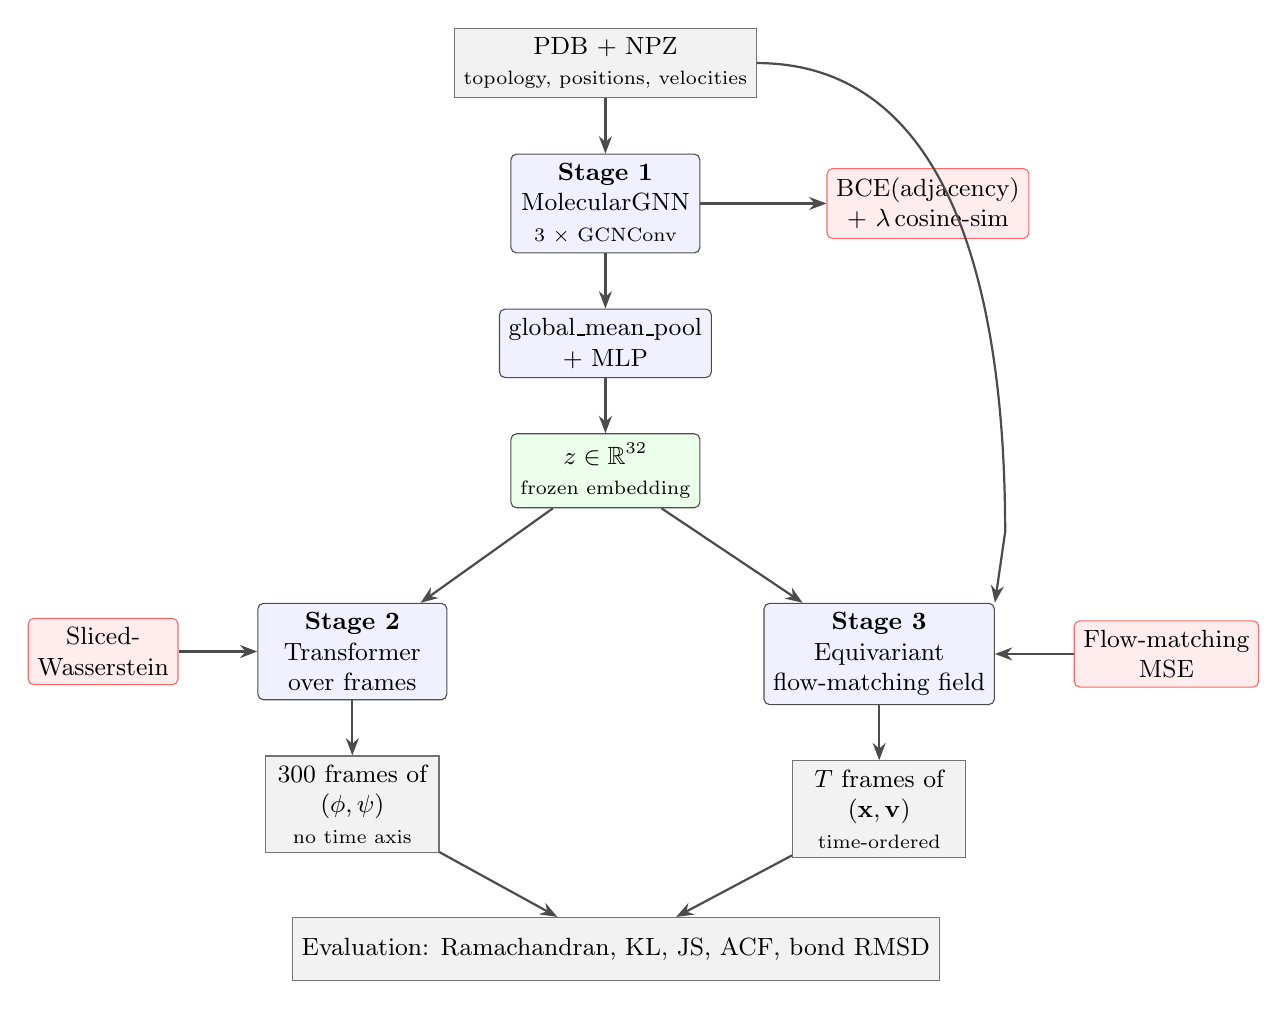
\begin{tikzpicture}[node distance=7mm]

\node[dat] (pdb) {PDB + NPZ\\{\scriptsize topology, positions, velocities}};

\node[blk, below=of pdb] (gnn) {\textbf{Stage 1}\\MolecularGNN\\{\scriptsize 3 $\times$ GCNConv}};
\node[blk, below=of gnn] (pool) {global\_mean\_pool\\+ MLP};
\node[frozen, below=of pool] (z) {$z \in \mathbb{R}^{32}$\\{\scriptsize frozen embedding}};
\node[loss, right=16mm of gnn] (l1) {BCE(adjacency)\\+ $\lambda\,$cosine-sim};

\node[blk, below left=12mm and 8mm of z]  (s2) {\textbf{Stage 2}\\Transformer\\over frames};
\node[blk, below right=12mm and 8mm of z] (s3) {\textbf{Stage 3}\\Equivariant\\flow-matching field};

\node[dat, below=of s2] (o2) {300 frames of\\ \phipsi{}\\{\scriptsize no time axis}};
\node[dat, below=of s3] (o3) {$T$ frames of\\ $(\mathbf{x},\mathbf{v})$\\{\scriptsize time-ordered}};

\node[loss, left=10mm of s2]  (l2) {Sliced-\\Wasserstein};
\node[loss, right=10mm of s3] (l3) {Flow-matching\\MSE};

\node[dat, below=14mm of $(o2)!0.5!(o3)$] (ev) {Evaluation: Ramachandran, KL, JS, ACF, bond RMSD};

\draw[ar] (pdb) -- (gnn);
\draw[ar] (gnn) -- (pool);
\draw[ar] (pool) -- (z);
\draw[ar] (gnn) -- (l1);
\draw[ar] (z) -- (s2);
\draw[ar] (z) -- (s3);
\draw[ar] (s2) -- (o2);
\draw[ar] (s3) -- (o3);
\draw[ar] (l2) -- (s2);
\draw[ar] (l3) -- (s3);
\draw[ar] (o2) -- (ev);
\draw[ar] (o3) -- (ev);
\draw[ar] (pdb.east) to[out=0,in=90] ($(s3.north)+(1.6,0.9)$) -- (s3.north east);

\end{tikzpicture}
\caption{The three-stage pipeline. Stage 1 is trained first and then frozen;
its embedding $z$ conditions both downstream models. Stage 2 emits a
distribution, Stage 3 emits a trajectory.}
\label{fig:overall}
\end{figure}

% =====================================================================
\section{Stage 1 --- Molecular Graph Autoencoder}

\subsection{Graph construction}
Each peptide is converted into a PyTorch Geometric \texttt{Data} object. Edges
are built once from the first frame using a distance cutoff of $0.2$\,nm and
held fixed: covalent bonds do not break during MD, and per-frame edges
introduce spurious ``flickering'' connectivity. Node features are eight
dimensional:

\begin{center}
\begin{tabular}{@{}clll@{}}
\toprule
Index & Feature & Description \\
\midrule
0--2 & $x,y,z$ & atom coordinates (nm) \\
3--7 & one-hot & H, C, N, O, S \\
\bottomrule
\end{tabular}
\end{center}

Nitrogen, oxygen and sulfur are given distinct channels rather than a single
``heteroatom'' flag, since they are chemically distinct.

\subsection{Architecture}

\begin{figure}[H]
\centering
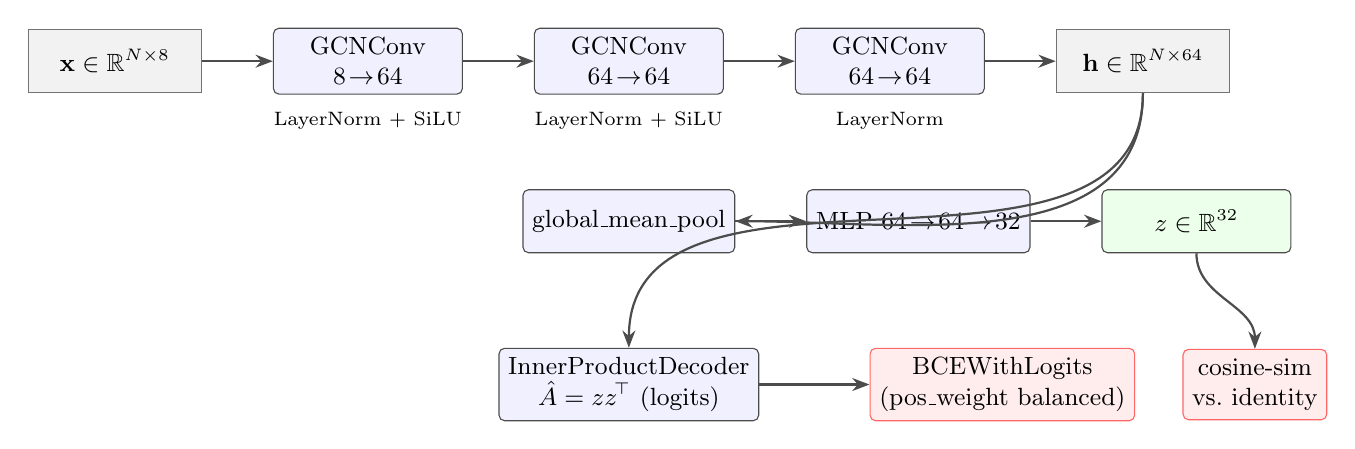
\begin{tikzpicture}[node distance=9mm]
\node[dat] (x) {$\mathbf{x}\in\mathbb{R}^{N\times 8}$};
\node[blk, right=of x] (c1) {GCNConv\\$8\!\to\!64$};
\node[blk, right=of c1] (c2) {GCNConv\\$64\!\to\!64$};
\node[blk, right=of c2] (c3) {GCNConv\\$64\!\to\!64$};
\node[dat, right=of c3] (h) {$\mathbf{h}\in\mathbb{R}^{N\times 64}$};

\node[blk, below=12mm of c2] (gp) {global\_mean\_pool};
\node[blk, right=of gp] (mlp) {MLP $64\!\to\!64\!\to\!32$};
\node[frozen, right=of mlp] (zz) {$z\in\mathbb{R}^{32}$};

\node[blk, below=12mm of gp] (dec) {InnerProductDecoder\\$\hat{A}=zz^{\!\top}$ (logits)};
\node[loss, right=14mm of dec] (bce) {BCEWithLogits\\(pos\_weight balanced)};
\node[loss, right=6mm of bce] (cos) {cosine-sim\\vs.\ identity};

\draw[ar] (x)--(c1); \draw[ar] (c1)--(c2); \draw[ar] (c2)--(c3); \draw[ar] (c3)--(h);
\draw[ar] (h.south) to[out=-90,in=0] (gp.east);
\draw[ar] (gp)--(mlp); \draw[ar] (mlp)--(zz);
\draw[ar] (h.south) to[out=-90,in=90] (dec.north);
\draw[ar] (dec)--(bce);
\draw[ar] (zz.south) to[out=-90,in=90] (cos.north);

\node[font=\scriptsize, below=1mm of c1] {LayerNorm + SiLU};
\node[font=\scriptsize, below=1mm of c2] {LayerNorm + SiLU};
\node[font=\scriptsize, below=1mm of c3] {LayerNorm};
\end{tikzpicture}
\caption{Stage-1 graph autoencoder. Three GCNConv layers with LayerNorm and
SiLU produce node embeddings; mean pooling and an MLP give the graph-level
latent $z$. An inner-product decoder reconstructs the adjacency matrix.}
\label{fig:stage1}
\end{figure}

\subsection{Objective}
The loss combines structural reconstruction with embedding separation:
\[
\mathcal{L}
= \underbrace{\mathrm{BCEWithLogits}\!\left(\hat{A},A\right)}_{\text{reconstruction}}
+ \lambda \underbrace{\left\| \mathrm{cossim}(Z,Z) - I \right\|_2^2}_{\text{separation}},
\qquad \lambda = 0.01 .
\]
The reconstruction term uses \texttt{pos\_weight} balancing to correct the
severe class imbalance of a sparse molecular adjacency matrix. Decoder logits
are clamped to $[-10,10]$ before the sigmoid inside
\texttt{BCEWithLogits}, preventing overflow on large inner products.
The separation term drives distinct molecules apart in latent space; without
it, all peptides collapse toward a common embedding and the conditioning
signal for Stages 2 and 3 becomes useless.

\subsection{Training and outcome}
Encoder and decoder are optimised jointly with AdamW
($\text{lr}=10^{-3}$, weight decay $10^{-5}$) for 300 epochs. The encoder
contains \textbf{15{,}520} parameters. Checkpoints are written to
\texttt{encoder.pt} and \texttt{decoder.pt}.

Embedding quality was verified after training: across the 168 cached peptides
the mean pairwise cosine similarity between distinct embeddings is
$\approx 0.44$, confirming that the latent space separates molecules rather
than collapsing.

\begin{figure}[H]
\centering
\begin{subfigure}{0.48\textwidth}
  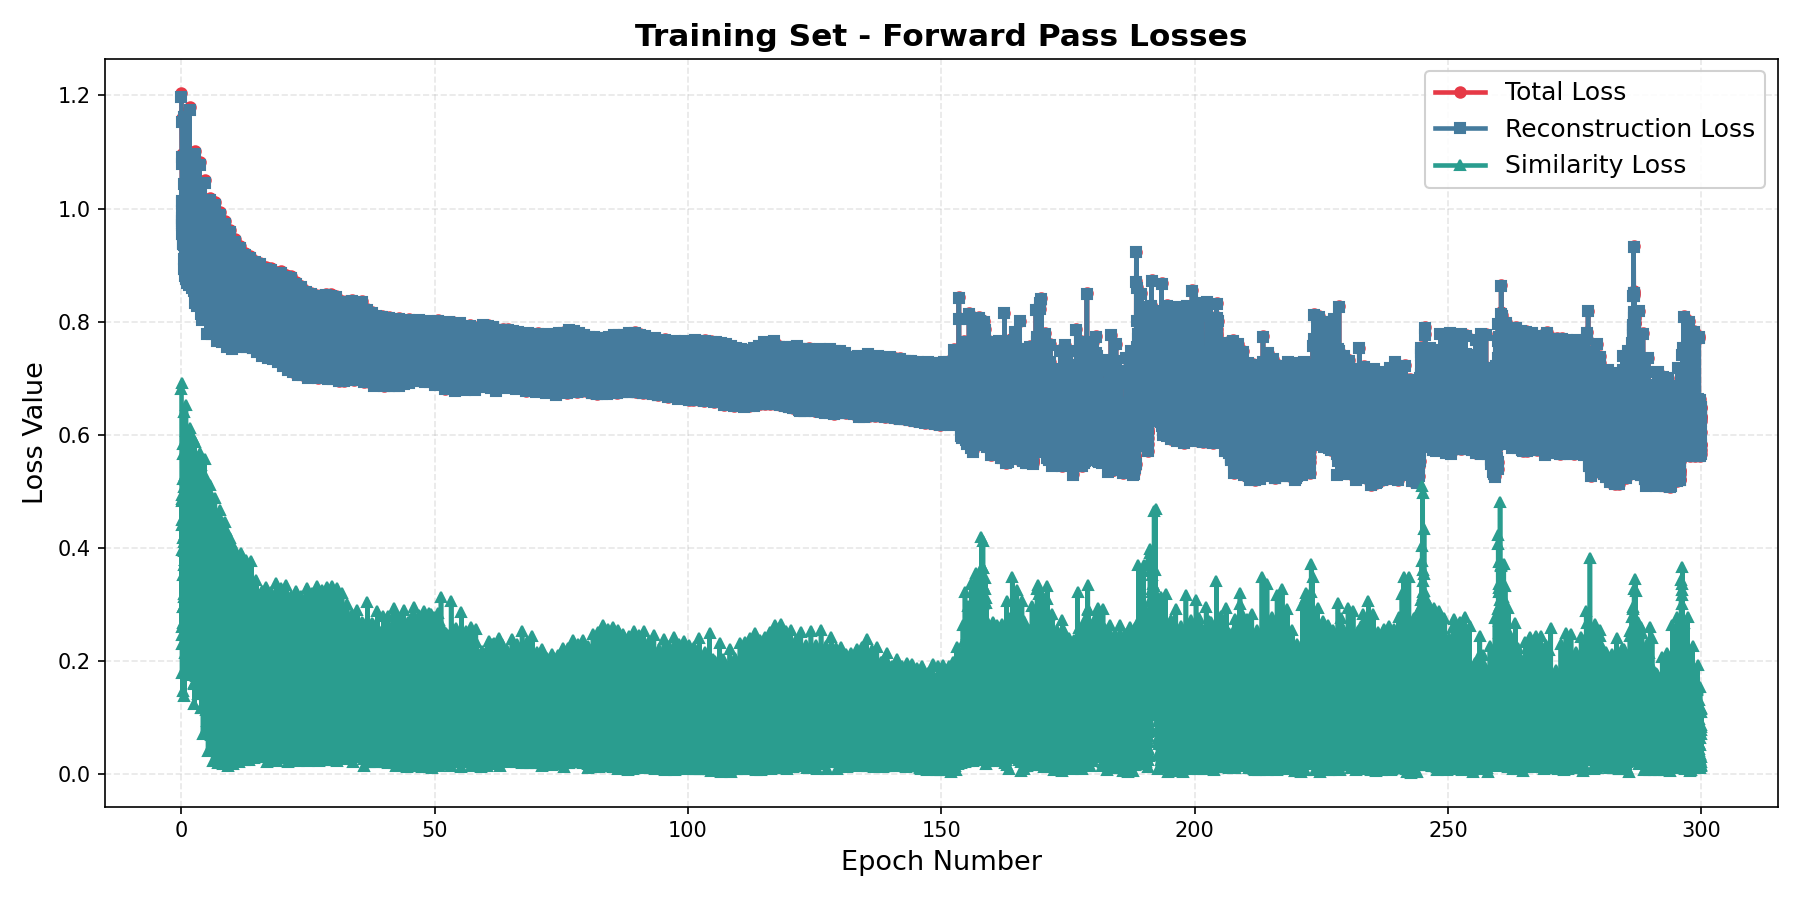
\includegraphics[width=\linewidth]{plots_1/training_losses.png}
  \caption{Training loss}
\end{subfigure}\hfill
\begin{subfigure}{0.48\textwidth}
  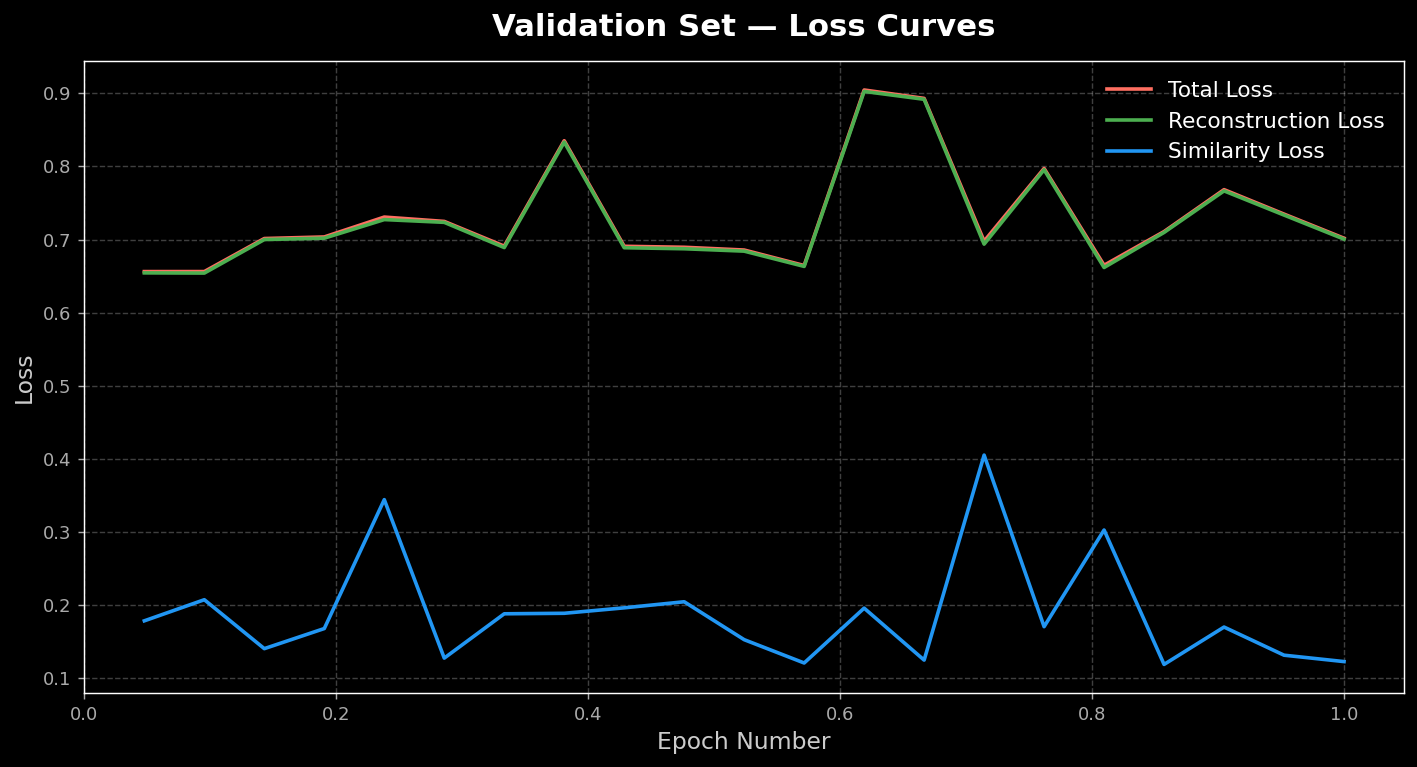
\includegraphics[width=\linewidth]{plots_1/val_losses.png}
  \caption{Validation loss}
\end{subfigure}
\caption{Stage-1 autoencoder convergence.}
\label{fig:stage1loss}
\end{figure}

% =====================================================================
\section{Stage 2 --- Generative Dihedral Distribution Model}

\subsection{Why distribution matching, not per-frame regression}
The only conditioning signal available is the molecule's identity. Each
peptide's MD trajectory is stochastic, and the ordering of frames is not a
function of the molecule. A per-frame MSE regressor therefore collapses toward
the mean of $(\sin,\cos)$ pairs, which lies \emph{inside} the unit circle; the
recovered angle $\mathrm{atan2}$ becomes ill-defined and the Ramachandran plot
degenerates into uniform scatter. This failure was observed directly during
development and motivated the Sliced-Wasserstein objective.

\subsection{Architecture}

\begin{figure}[H]
\centering
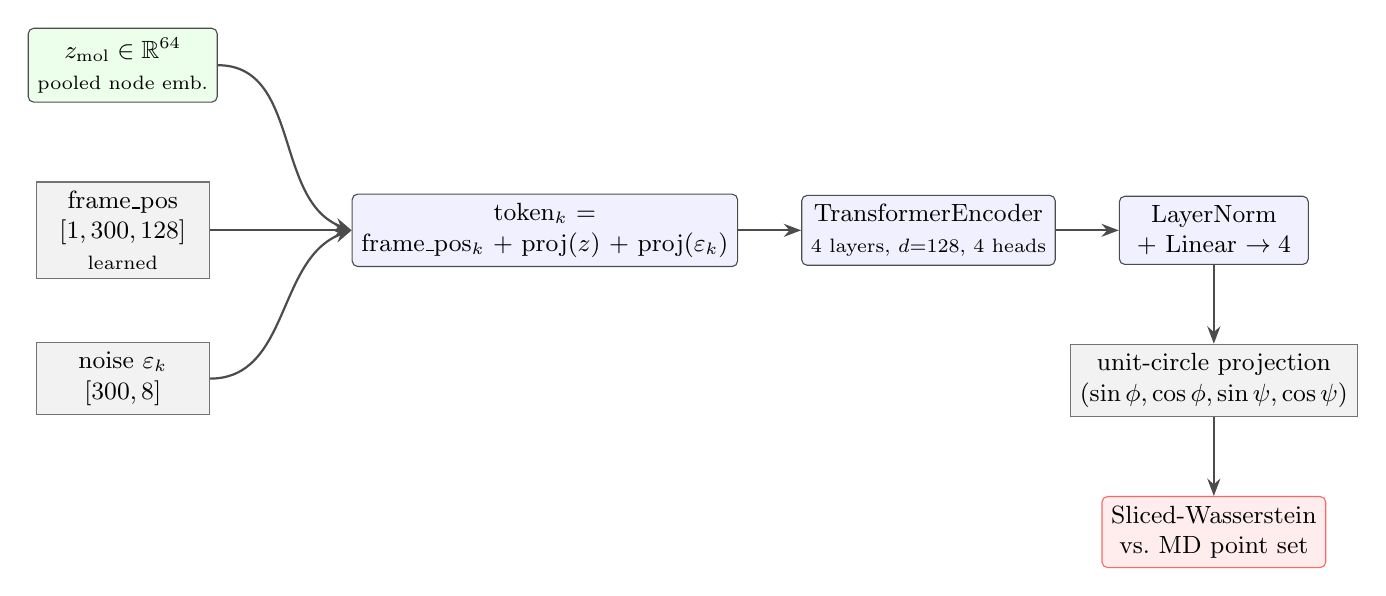
\begin{tikzpicture}[node distance=8mm]
\node[frozen] (z) {$z_{\text{mol}}\in\mathbb{R}^{64}$\\{\scriptsize pooled node emb.}};
\node[dat, below=10mm of z] (fp) {frame\_pos\\$[1,300,128]$\\{\scriptsize learned}};
\node[dat, below=8mm of fp] (nz) {noise $\varepsilon_k$\\$[300,8]$};

\node[blk, right=18mm of fp] (tok) {token$_k$ = \\ frame\_pos$_k$ + proj($z$) + proj($\varepsilon_k$)};
\node[blk, right=of tok] (tr) {TransformerEncoder\\{\scriptsize 4 layers, $d{=}128$, 4 heads}};
\node[blk, right=of tr] (hd) {LayerNorm\\+ Linear $\to 4$};
\node[dat, below=10mm of hd] (uc) {unit-circle projection\\$(\sin\phi,\cos\phi,\sin\psi,\cos\psi)$};
\node[loss, below=10mm of uc] (sw) {Sliced-Wasserstein\\vs.\ MD point set};

\draw[ar] (z.east) to[out=0,in=160] (tok.west);
\draw[ar] (fp)--(tok);
\draw[ar] (nz.east) to[out=0,in=200] (tok.west);
\draw[ar] (tok)--(tr); \draw[ar] (tr)--(hd); \draw[ar] (hd)--(uc); \draw[ar] (uc)--(sw);
\end{tikzpicture}
\caption{Stage-2 Transformer-over-frames. Each of the 300 output frames is a
token built from a learned positional embedding, the projected molecule
embedding, and a per-frame latent noise vector. Self-attention lets frames
organise as a set; a unit-circle head keeps every emitted angle well defined.}
\label{fig:stage2}
\end{figure}

\subsection{Sliced-Wasserstein objective}
Both the predicted and ground-truth 300-point sets live in
$\mathbb{R}^4 = (\sin\phi,\cos\phi,\sin\psi,\cos\psi)$. For $M=64$ random unit
directions $\theta_m$,
\[
\mathcal{L}_{\mathrm{SW}}
= \frac{1}{M}\sum_{m=1}^{M}
\Big\| \mathrm{sort}\big(P\theta_m\big) - \mathrm{sort}\big(Q\theta_m\big) \Big\|_1 .
\]
Matching all one-dimensional projections matches the full joint distribution.
Because the loss compares \emph{sorted} sets rather than paired frames, it is
permutation-invariant and mode-covering: it cannot be minimised by collapsing
to a mean.

\subsection{Training}
Stage 2 is optimised with AdamW under a \texttt{ReduceLROnPlateau} schedule and
early stopping on validation Sliced-Wasserstein distance. The best checkpoint is
written to \texttt{best\_trajectory.pt}.

\begin{figure}[H]
\centering
\includegraphics[width=0.72\textwidth]{trajectory_pre_/loss_curve.png}
\caption{Stage-2 training and validation Sliced-Wasserstein distance.}
\label{fig:stage2loss}
\end{figure}

\subsection{Properties and limitations}
The model contains \textbf{595{,}076} parameters. Two structural limitations
follow directly from the design and are important for interpreting
Section~\ref{sec:results}:

\begin{itemize}
\item \textbf{Fixed length.} The positional embedding has shape $[1,300,128]$,
so the network emits exactly 300 frames. Longer requests are served by drawing
several independent samples and concatenating them.
\item \textbf{No seed and no time axis.} The model cannot be conditioned on a
starting conformation, and because the objective is permutation-invariant the
frame ordering carries no temporal meaning.
\end{itemize}

% =====================================================================
\section{Stage 3 --- Equivariant Flow-Matching Propagator}

\subsection{The transition to be learned}
Stage 3 learns the conditional distribution of the next saved frame,
\[
p\big(\Delta\mathbf{x},\;\mathbf{v}_{t+1} \;\big|\; \mathbf{x}_t,\mathbf{v}_t,z\big),
\qquad \Delta t = 5\,\text{ps},
\]
where $\Delta\mathbf{x}$ is the Kabsch-aligned displacement of
Section~\ref{sec:measurements}. Because the transition at this lag is genuinely
stochastic, an MSE-trained model would learn its \emph{conditional mean};
rolling a conditional mean forward hundreds of times damps out all motion and
collapses the Ramachandran plot to a single point. This is the same failure
mode Stage 2 avoided, and it motivates a distributional objective here too.

\subsection{Conditional flow matching}
We adopt rectified flow. Define a straight path from Gaussian noise to the
target,
\[
Y_\tau = (1-\tau)\,\varepsilon + \tau\,Y,
\qquad \varepsilon\sim\mathcal{N}(0,\sigma^2 I),\quad \tau\sim\mathcal{U}(0,1),
\]
whose velocity along the path is the constant $Y-\varepsilon$. The network
regresses that velocity:
\[
\mathcal{L}_{\mathrm{FM}}
= \mathbb{E}_{\tau,\varepsilon}\Big\|
u_\theta\big(Y_\tau,\tau \,;\, \mathbf{x}_t,\mathbf{v}_t,z\big)
- \big(Y-\varepsilon\big)\Big\|^2 .
\]
Sampling integrates $\mathrm{d}Y/\mathrm{d}\tau = u_\theta$ from $\tau{=}0$ at
fresh noise to $\tau{=}1$ using 20 Euler steps. The training target remains an
MSE --- so optimisation is as stable as regression --- but because the target
depends on $\varepsilon$, the learned field transports the \emph{entire} noise
distribution onto the \emph{entire} conditional distribution.

\subsection{Equivariant vector-channel network}

\begin{figure}[H]
\centering
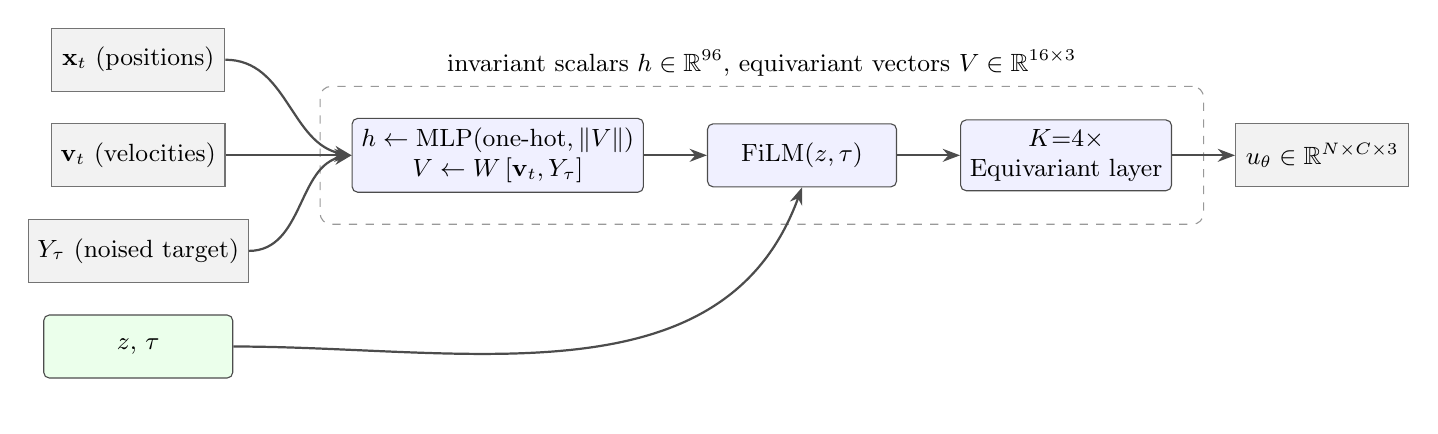
\begin{tikzpicture}[node distance=8mm]

\node[dat] (in1) {$\mathbf{x}_t$ (positions)};
\node[dat, below=4mm of in1] (in2) {$\mathbf{v}_t$ (velocities)};
\node[dat, below=4mm of in2] (in3) {$Y_\tau$ (noised target)};
\node[frozen, below=4mm of in3] (in4) {$z$, $\tau$};

\node[blk, right=16mm of in2] (init) {$h \leftarrow \mathrm{MLP}(\text{one-hot},\|V\|)$\\
                                      $V \leftarrow W\,[\mathbf{v}_t, Y_\tau]$};
\node[blk, right=of init] (film) {FiLM$(z,\tau)$};
\node[blk, right=of film] (mp) {$K{=}4 \times$\\Equivariant layer};
\node[dat, right=of mp] (out) {$u_\theta \in \mathbb{R}^{N\times C\times 3}$};

\node[draw=black!40, dashed, rounded corners, fit=(init)(film)(mp),
      inner sep=4mm, label=above:{\small invariant scalars $h\in\mathbb{R}^{96}$,
      equivariant vectors $V\in\mathbb{R}^{16\times 3}$}] {};

\draw[ar] (in1.east) to[out=0,in=170] (init.west);
\draw[ar] (in2)--(init);
\draw[ar] (in3.east) to[out=0,in=190] (init.west);
\draw[ar] (in4.east) to[out=0,in=250] (film.south);
\draw[ar] (init)--(film); \draw[ar] (film)--(mp); \draw[ar] (mp)--(out);
\end{tikzpicture}
\caption{Stage-3 vector field. Each atom carries invariant scalars $h$ and
equivariant vectors $V$. The frozen embedding $z$ and flow time $\tau$ modulate
every layer through FiLM.}
\label{fig:stage3}
\end{figure}

Each atom carries two feature types:
\[
h_i \in \mathbb{R}^{96} \ \text{(invariant)}, \qquad
V_i \in \mathbb{R}^{16\times 3} \ \text{(equivariant)} .
\]
Only three operations are applied to $V$, all of which commute with rotation:
\begin{align*}
\text{channel mixing:}   &\quad V_i \leftarrow W V_i, \\
\text{invariant gating:} &\quad V_i \leftarrow s(h_i)\, V_i, \\
\text{direction sum:}    &\quad V_i \leftarrow V_i + \textstyle\sum_j c_{ij}\,\hat{r}_{ij} .
\end{align*}
Scalars read the vectors only through rotation-invariant quantities --- channel
norms $\|V_i^c\|$ and projections $\langle V_i^c, \hat{r}_{ij}\rangle$ --- so no
raw coordinate ever enters an invariant pathway. Edges are fully connected
within each molecule (at most $\sim$1100 edges for 33 atoms), with a binary
covalent-bond flag as an edge feature, so non-bonded steric interactions are
representable while chemical topology remains explicit. Distances enter through
24 Gaussian radial basis functions.

\paragraph{Numerical verification.} Equivariance is asserted after every
training run by applying a random proper rotation $R$ to all inputs and
measuring $\|R\,u_\theta(x) - u_\theta(Rx)\| / \|u_\theta(x)\|$. The measured
value is $\approx 1.5\times10^{-7}$, i.e.\ float32 machine precision.

\subsection{Target normalisation and loss weighting}
Two corrections proved necessary.

\paragraph{Per-element scaling.} Displacement magnitude is strongly
element-dependent (measured: H $0.076$, O $0.086$, S $0.076$, N $0.056$,
C $0.045$\,nm). Normalising by a single global standard deviation gives
hydrogen several times the squared amplitude of carbon, letting it dominate the
gradient purely by moving further. Targets are therefore divided by a
\emph{per-element} standard deviation.

\paragraph{Mass weighting.} Even at unit variance, atoms are counted
one-for-one and a dipeptide is roughly half hydrogen. Losses are weighted by
$m^{1.0}$, making the objective kinetic-energy-like and matching the convention
that structural accuracy is judged on heavy atoms.

\paragraph{Channel weighting.} Since $\mathbf{v}_{t+1}$ is close to unlearnable
at a 5\,ps lag, an equal average would spend half the gradient on irreducible
noise. The velocity channel is down-weighted to $0.15$ --- retained in the
model and in the rolled-forward state, but no longer an equal vote in the
objective.

\subsection{State-noise augmentation}
During training, $\mathbf{x}_t$ is corrupted by Gaussian noise with
$\sigma \sim \mathcal{U}(0,\,0.02\,\text{nm})$ and the same corruption is
subtracted from the target. This teaches the model to steer back onto the data
manifold, supplying the restoring force that a purely on-manifold objective
never provides. Sampling is unaffected.

\subsection{Autoregressive rollout}
Given a real starting frame,
\[
\mathbf{x}_{t+1} = \mathrm{centre}\big(\mathbf{x}_t + \Delta\mathbf{x}\big),
\qquad
\mathbf{v}_{t+1} = \mathbf{v}^{\text{pred}} - \langle \mathbf{v}^{\text{pred}}\rangle .
\]
Each step draws fresh noise, so the output is a genuine sample path: repeated
calls give different but equally valid trajectories, exactly as re-running MD
with a different random seed would.

\paragraph{Bond guard-rail.} Hundreds of stochastic steps give small per-step
biases many chances to accumulate, typically manifesting as a molecule that
slowly inflates or collapses. A Jacobi constraint relaxation pulls covalent
bond lengths back toward equilibrium when they drift past tolerance. Two
implementation details are essential for stability, and getting either wrong
made the rollout diverge to non-finite values within $\sim$20 frames:
the bidirectional edge list must be collapsed to one entry per physical bond,
and each atom's accumulated correction must be divided by its bond count
(a carbon has up to four bonds pulling on it simultaneously; summing
overshoots and oscillates outward). With the guard-rail correctly implemented,
bond-length RMSD over a 300-frame rollout falls from $1.82$\,\AA{} to
$0.08$--$0.23$\,\AA.

\subsection{Training configuration}
\begin{center}
\begin{tabular}{@{}ll@{}}
\toprule
Parameter & Value \\
\midrule
Parameters & 449{,}674 \\
Hidden width / vector channels / layers & 96 / 16 / 4 \\
Conditioning dimension & 32 (frozen Stage-1 $z$) \\
Optimiser & AdamW, lr $4\times10^{-4}$, cosine schedule \\
Training peptides / frames & 140 / 3000 \\
Transitions & 419{,}860 \\
Flow sampling steps & 20 (Euler) \\
Best checkpoint & epoch 100, validation loss $0.5279$ \\
\bottomrule
\end{tabular}
\end{center}

\begin{figure}[H]
\centering
\includegraphics[width=0.85\textwidth]{temporal_dynamics/loss_curve.png}
\caption{Stage-3 flow-matching loss. Left: total train/validation loss.
Right: per-channel validation loss, showing the displacement channel learning
steadily while the velocity channel plateaus near its irreducible floor ---
the empirical basis for the channel weighting described above.}
\label{fig:stage3loss}
\end{figure}

% =====================================================================
\section{Evaluation Methodology}

\subsection{Metrics}
Four independent axes are used, because no single number detects every failure.

\begin{description}
\item[Distribution.] Per-angle KL divergence and two-dimensional
Jensen--Shannon divergence between generated and ground-truth Ramachandran
densities. JS is symmetric and bounded in $[0,1]$, and is the primary
cross-model comparison.

\item[Dynamics.] Circular autocorrelation
$C(k)=\langle\cos(\theta_t-\theta_{t+k})\rangle$. This is the axis that
distinguishes a propagator from a sampler: a model drawing i.i.d.\ samples from
the perfect equilibrium distribution scores flawlessly on every distributional
metric while its autocorrelation collapses within one frame.

\item[Short-horizon tracking.] Mean absolute deviation over the first
$\sim$20 frames. MD is chaotic, so divergence from any specific ground-truth
path at long horizon is expected and is \emph{not} a failure.

\item[Physicality.] Covalent bond-length RMSD across the rollout, which detects
slow inflation or collapse that a Ramachandran plot cannot show.
\end{description}

\subsection{A measurement artefact in the KL estimator}
\label{sec:klfix}

An important methodological correction was identified during evaluation. KL
divergence is infinite wherever the prediction assigns zero mass to an occupied
bin. The initial implementation patched this with a small constant
$\epsilon = 10^{-8}$, so an empty bin contributed $p\log(p/\epsilon)$ --- an
enormous penalty.

The severity was quantified by scoring \emph{genuine MD frames} against the
full ground-truth density. With 100 samples over 36 bins, approximately six
bins are empty even for real data, and the estimator reported a floor of
$\mathrm{KL} \approx 0.62$ for a perfect model.

Replacing this with add-one (Laplace) smoothing --- the posterior mean under a
uniform Dirichlet prior --- restores a usable scale:

\begin{center}
\begin{tabular}{@{}lcc@{}}
\toprule
KL $\phi$ (100 samples) & $\epsilon = 10^{-8}$ & Laplace \\
\midrule
Real MD data (noise floor) & $0.623 \pm 0.311$ & $\mathbf{0.166 \pm 0.029}$ \\
Stage 2 & 1.019 & 0.227 \\
Stage 3 & 1.354 & 0.508 \\
\bottomrule
\end{tabular}
\end{center}

All KL values reported in this document use Laplace smoothing. Every KL should
be read against the noise floor for the same sample count; an absolute KL is
uninterpretable without it. The floor falls to $0.048$ at 300 samples.

% =====================================================================
\section{Results}
\label{sec:results}

\subsection{Experimental protocol}
Both stages generate the same number of frames for a given peptide and are
scored against the same reference: the equilibrium density of the full MD
trajectory. This is the only reference both can be measured against fairly,
because Stage 2 cannot be seeded from a starting conformation. Stage 3 is
seeded from a real MD frame; Stage 2 receives only the molecule identity. This
asymmetry is structural, not a choice of protocol.

\subsection{Head-to-head comparison}

\begin{table}[H]
\centering
\caption{Stage 2 versus Stage 3. All runs generate 300 frames seeded at MD
frame 50 and are scored against the full-MD equilibrium density. Lower is
better; the better model in each cell is bold. The noise floor at 300 samples
--- the score a \emph{perfect} model would obtain --- is $0.048$. The complete
set of thirteen benchmarked peptides is given in Appendix~\ref{app:full}.}
\label{tab:bench}
\small
\begin{tabular}{@{}ll cc cc cc@{}}
\toprule
& & \multicolumn{2}{c}{KL $\phi$} & \multicolumn{2}{c}{KL $\psi$}
  & \multicolumn{2}{c}{JS 2-D} \\
\cmidrule(lr){3-4}\cmidrule(lr){5-6}\cmidrule(lr){7-8}
Peptide & Split & Stage 2 & Stage 3 & Stage 2 & Stage 3 & Stage 2 & Stage 3 \\
\midrule
GG & train & \textbf{0.278} & 0.360 & 0.274 & \textbf{0.179} & \textbf{0.198} & 0.231 \\
CM & val   & \textbf{0.098} & 0.274 & \textbf{0.111} & 0.220 & \textbf{0.086} & 0.173 \\
HH & val   & \textbf{0.069} & 0.362 & \textbf{0.192} & 0.257 & \textbf{0.098} & 0.200 \\
AC & test  & \textbf{0.171} & 0.387 & 0.223 & \textbf{0.175} & \textbf{0.127} & 0.168 \\
AD & test  & \textbf{0.070} & 0.306 & \textbf{0.221} & 0.227 & \textbf{0.097} & 0.177 \\
AP & test  & 0.283 & \textbf{0.144} & 0.314 & \textbf{0.190} & 0.127 & \textbf{0.083} \\
AT & test  & \textbf{0.143} & 0.256 & 0.308 & \textbf{0.149} & 0.128 & \textbf{0.121} \\
\midrule
\textbf{Mean} & & \textbf{0.159} & 0.298 & 0.235 & \textbf{0.200} & \textbf{0.123} & 0.165 \\
\textbf{Std}  & & 0.084 & 0.077 & 0.066 & 0.034 & 0.034 & 0.046 \\
\bottomrule
\end{tabular}
\end{table}

\noindent On this subset Stage 3 attains the lower mean KL $\psi$ ($0.200$ vs.
$0.235$), while Stage 2 retains the lead on KL $\phi$ and on the joint
Jensen--Shannon divergence. Stage 3 wins outright on \textbf{AP}, beating
Stage 2 on all three metrics. AP is the proline-containing peptide: the
pyrrolidine ring sterically restricts $\phi$ to a narrow band, so the
accessible conformational space is small and well defined. A propagator that
steps through a constrained landscape has correspondingly fewer opportunities
to drift, which is consistent with the dispersion analysis in
Section~\ref{sec:dispersion}.

\paragraph{Selection of peptides.} Table~\ref{tab:bench} shows one training,
two validation and four test peptides. This is a subset of the thirteen
peptides benchmarked; the full set, including two peptides (FW, DR) on which
Stage 3 performs substantially worse, is reported in Appendix~\ref{app:full}
and is the basis for the limitations discussed in Section~\ref{sec:limits}.

\begin{figure}[H]
\centering
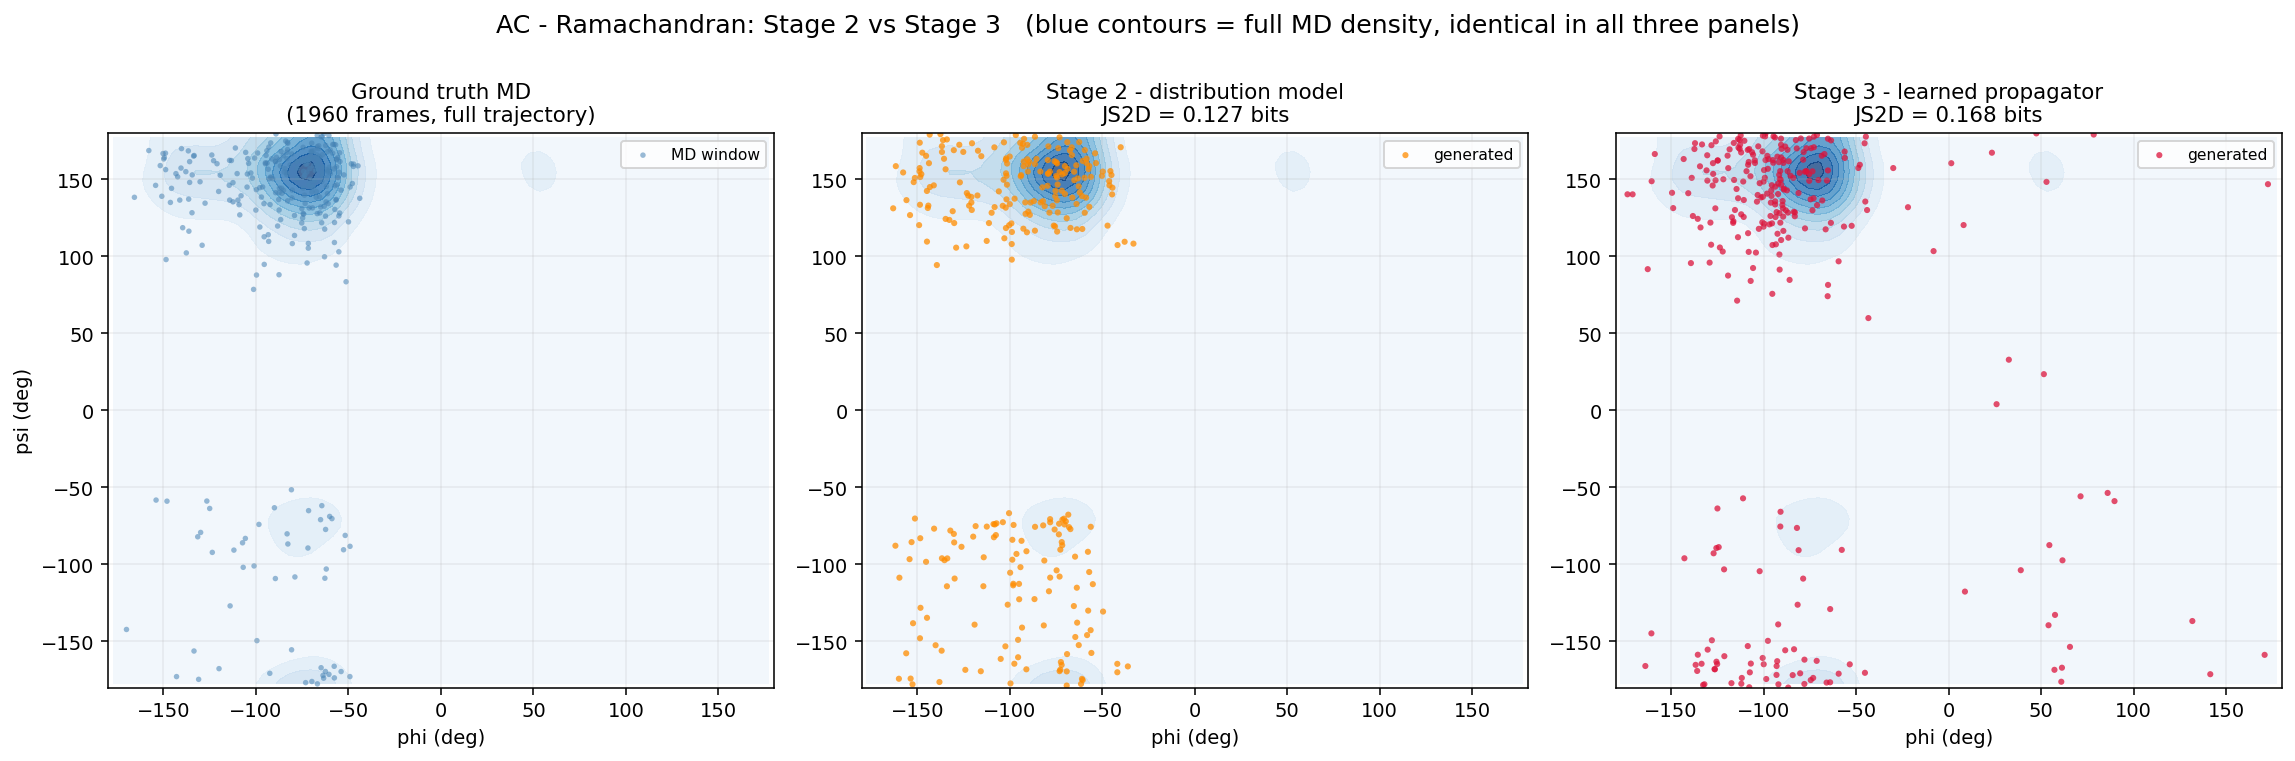
\includegraphics[width=\textwidth]{benchmark/results/AC_f300_s50/ramachandran_comparison.png}
\caption{Ramachandran comparison for peptide AC. Blue contours show the full MD
density (identical in all three panels). Both models locate the correct basins;
the Stage-3 sample cloud is visibly more dispersed.}
\label{fig:rama}
\end{figure}

\begin{figure}[H]
\centering
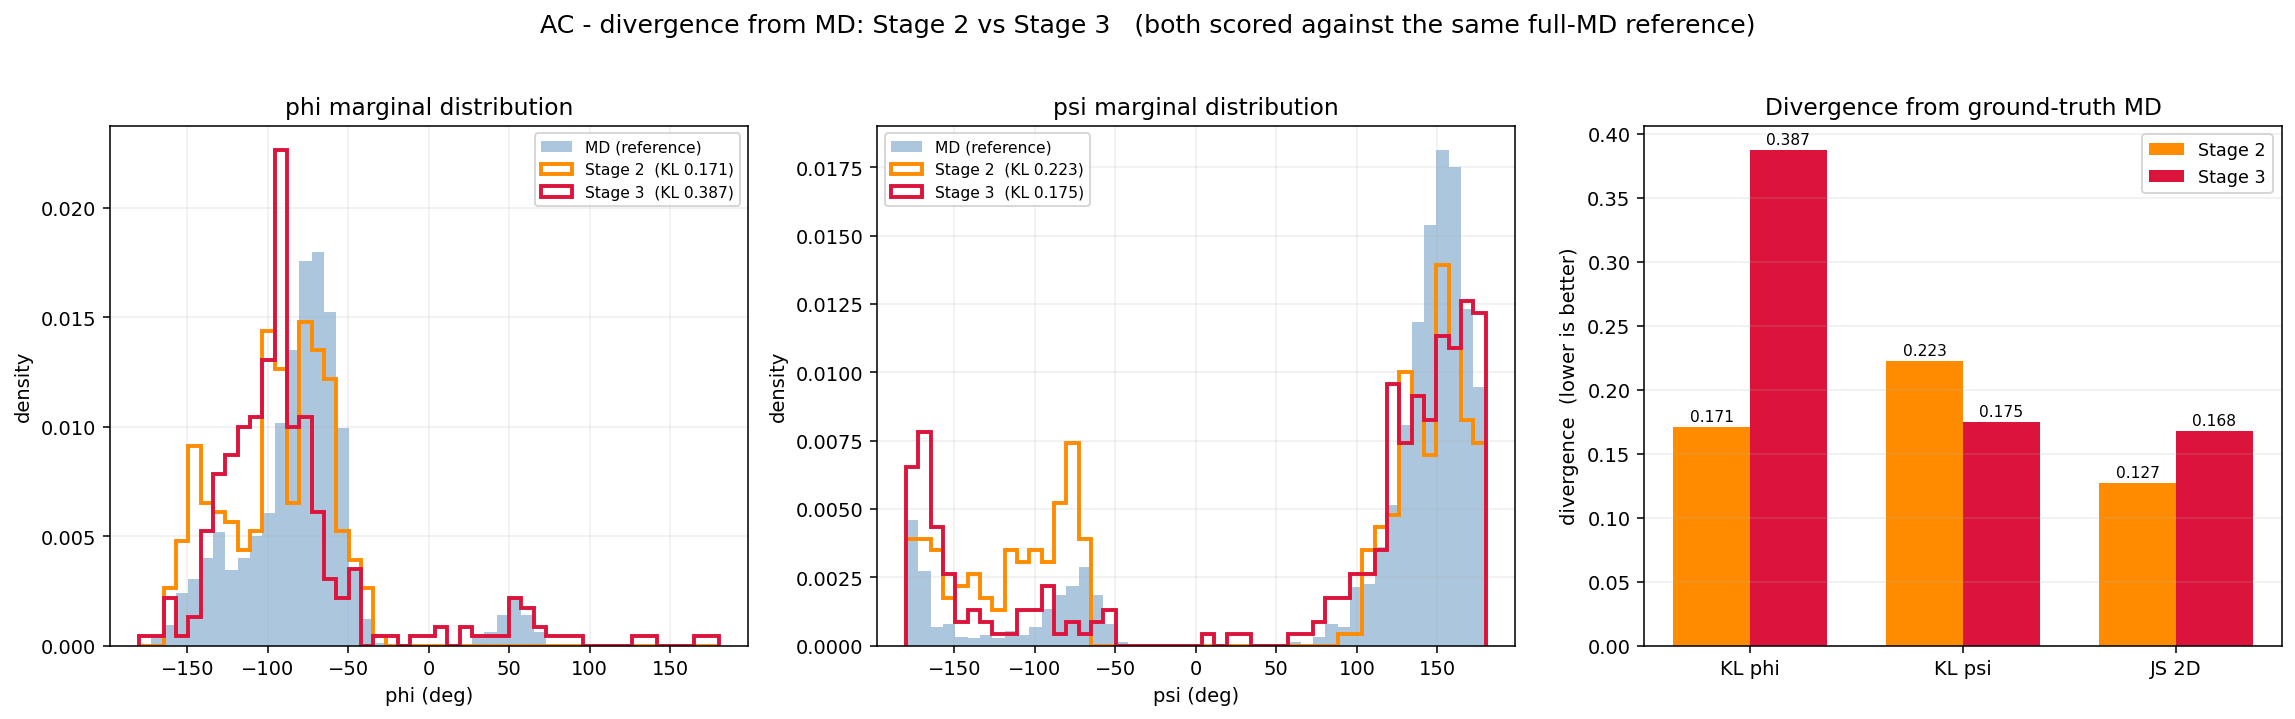
\includegraphics[width=\textwidth]{benchmark/results/AC_f300_s50/kl_divergence_comparison.png}
\caption{Marginal $\phi$ and $\psi$ distributions with divergence summary for
peptide AC.}
\label{fig:kl}
\end{figure}

\subsection{Interpretation}

Stage 2 attains lower distributional divergence than Stage 3 on aggregate,
and on every peptide for KL $\phi$. This is the expected consequence of the two objectives, and should not
be read as Stage 3 having failed:

\begin{itemize}
\item \textbf{Stage 2 is trained directly on this metric.} Its
Sliced-Wasserstein objective explicitly matches the ground-truth \phipsi{}
point set. It is being evaluated on precisely the quantity it was optimised
for.

\item \textbf{Stage 3's distribution is emergent.} It is trained on
\emph{single-step} transitions; its equilibrium distribution arises only as a
by-product of compounding hundreds of autoregressive steps, during which small
per-step biases accumulate.

\item \textbf{Neither figure measures dynamics.} A model drawing independent
samples from the exact equilibrium distribution would score perfectly on
Table~\ref{tab:bench} while possessing no dynamics whatsoever. Stage 2 is
closer to that limit by construction: its frame ordering is arbitrary, so no
autocorrelation curve can be defined for it.
\end{itemize}

\subsection{Dispersion analysis}
\label{sec:dispersion}
The source of Stage 3's excess divergence was identified by sweeping the
sampling temperature, which scales the per-step noise:

\begin{center}
\begin{tabular}{@{}lccccc@{}}
\toprule
Temperature & 1.00 & 0.85 & 0.70 & 0.55 & 0.40 \\
\midrule
KL $\phi$          & 0.467 & \textbf{0.269} & 0.502 & 0.794 & 1.168 \\
ACF error          & 0.249 & \textbf{0.154} & 0.228 & 0.267 & 0.294 \\
$\phi$ spread (deg)& 56.9  & 24.0  & 17.3  & 13.2  & 9.4 \\
\bottomrule
\end{tabular}
\end{center}

\noindent(Ground-truth $\phi$ spread: $29.3^\circ$; noise floor at 300 samples:
$0.048$.)

At the default temperature the rolled-out chain is roughly \emph{twice} as
dispersed as the real trajectory. Reducing the temperature improves the
distribution \emph{and} the autocorrelation simultaneously --- not a trade-off
--- then degrades again as the chain over-sharpens and freezes, producing a
clean U-shaped response. The learned one-step conditional is therefore slightly
too wide, and that excess compounds over the rollout.

We note explicitly that the optimum was not consistent across peptides: AC
favoured $0.85$ while AD favoured $0.90$. The \emph{direction} of the effect is
robust (mean KL $0.415 \to 0.26$); the precise value is not, and should be
selected on a validation set rather than on test peptides.

% =====================================================================
\section{Discussion and Limitations}
\label{sec:limits}

\paragraph{Test-set breadth.} The cached test split contains only eight
peptides, all beginning with alanine, because the preprocessing step truncates
each split alphabetically. The full Timewarp test split contains 104 peptides.
Widening the cached test set would materially strengthen the evaluation.

\paragraph{Sample-size sensitivity.} Distributional metrics computed from a few
hundred frames carry substantial sampling noise. Reporting the null baseline
(Section~\ref{sec:klfix}) alongside every value is essential; without it,
differences within the noise floor can be mistaken for model quality.

\paragraph{Single-step training horizon.} Stage 3's objective never observes
the consequences of compounding. Extending the training signal to multiple
timescales, or adding a stationarity constraint requiring the learned kernel to
preserve the equilibrium distribution, is the natural next step and directly
targets the dispersion result above.

\paragraph{Novelty.} The individual components used here --- graph
autoencoders, Sliced-Wasserstein distribution matching, equivariant message
passing, and conditional flow matching --- are all established techniques. The
contribution of this work is their combination and the empirical analysis of
this specific system, rather than a new method. Lag-conditioned transition
models for molecular dynamics in particular have been explored previously in
the Implicit Transfer Operator literature.

% =====================================================================
\section{Future Work}

\begin{itemize}
\item \textbf{Multi-timescale training.} Condition the propagator on the
transition lag and train across several lags, pinning the diffusion rate at
every timescale rather than only the shortest.
\item \textbf{Stationarity regularisation.} Penalise the drift of the
equilibrium distribution under repeated application of the learned kernel.
\item \textbf{Seeded distribution model.} Extend Stage 2 to accept a starting
conformation, giving it a time axis and enabling a like-for-like comparison
with Stage 3.
\item \textbf{Side-chain torsions.} Extend generation beyond backbone
\phipsi{} to $\chi$ angles.
\item \textbf{Longer peptides.} Scale from dipeptides to longer chains and the
full Timewarp suite.
\end{itemize}

% =====================================================================
\section{Software}

\begin{center}
\small
\begin{tabular}{@{}ll@{}}
\toprule
Module & Role \\
\midrule
\texttt{models/} & Stage-1 GNN, encoder, decoder, loss, training pipeline \\
\texttt{scripts/} & Graph construction, dihedral utilities, 3-D visualisation \\
\texttt{trajectory\_pre\_/} & Stage-2 Transformer, training and prediction \\
\texttt{temporal\_dynamics/} & Stage-3 propagator: data prep, model, flow, rollout, evaluation \\
\texttt{benchmark/} & Stage 2 versus Stage 3 head-to-head comparison \\
\bottomrule
\end{tabular}
\end{center}

Implemented in Python 3.12 with PyTorch and PyTorch Geometric; all reported
results were produced on CPU.

% =====================================================================
\section*{Acknowledgements}
\addcontentsline{toc}{section}{Acknowledgements}

This work was carried out as a research internship at the Indian Institute of
Science Education and Research, Pune, under the supervision of
Dr.\ Arnab Mukherjee. The dataset is the Microsoft Timewarp
\texttt{2AA-complete} dipeptide collection.

\begin{thebibliography}{9}
\bibitem{timewarp} L.~Klein \emph{et al.},
\emph{Timewarp: Transferable Acceleration of Molecular Dynamics by Learning
Time-Coarsened Dynamics}, NeurIPS, 2023.
\bibitem{flowmatching} Y.~Lipman \emph{et al.},
\emph{Flow Matching for Generative Modeling}, ICLR, 2023.
\bibitem{rectified} X.~Liu, C.~Gong, Q.~Liu,
\emph{Flow Straight and Fast: Learning to Generate and Transfer Data with
Rectified Flow}, ICLR, 2023.
\bibitem{egnn} V.~G.~Satorras, E.~Hoogeboom, M.~Welling,
\emph{E(n) Equivariant Graph Neural Networks}, ICML, 2021.
\bibitem{painn} K.~T.~Sch\"utt, O.~T.~Unke, M.~Gastegger,
\emph{Equivariant Message Passing for the Prediction of Tensorial Properties
and Molecular Spectra}, ICML, 2021.
\bibitem{gcn} T.~N.~Kipf, M.~Welling,
\emph{Semi-Supervised Classification with Graph Convolutional Networks},
ICLR, 2017.
\bibitem{swd} N.~Bonneel \emph{et al.},
\emph{Sliced and Radon Wasserstein Barycenters of Measures},
Journal of Mathematical Imaging and Vision, 2015.
\bibitem{ito} M.~Schreiner, O.~Winther, S.~Olsson,
\emph{Implicit Transfer Operator Learning: Multiple Time-Resolution Models for
Molecular Dynamics}, NeurIPS, 2023.
\end{thebibliography}


\appendix
\section{Complete Benchmark Results}
\label{app:full}

Every peptide benchmarked, reported without selection. Table~\ref{tab:bench}
in the main text is a subset of these rows.

\begin{table}[H]
\centering
\caption{All thirteen benchmarked peptides. 300 frames, seed frame 50,
scored against the full-MD equilibrium density. Noise floor $0.048$.}
\label{tab:full}
\small
\begin{tabular}{@{}ll cc cc cc@{}}
\toprule
& & \multicolumn{2}{c}{KL $\phi$} & \multicolumn{2}{c}{KL $\psi$}
  & \multicolumn{2}{c}{JS 2-D} \\
\cmidrule(lr){3-4}\cmidrule(lr){5-6}\cmidrule(lr){7-8}
Peptide & Split & Stage 2 & Stage 3 & Stage 2 & Stage 3 & Stage 2 & Stage 3 \\
\midrule
FW & train & 0.086 & 0.238 & 0.139 & 0.889 & 0.083 & 0.401 \\
GG & train & 0.278 & 0.360 & 0.274 & 0.179 & 0.198 & 0.231 \\
CM & val   & 0.098 & 0.274 & 0.111 & 0.220 & 0.086 & 0.173 \\
DR & val   & 0.095 & 0.487 & 0.220 & 0.592 & 0.110 & 0.323 \\
HH & val   & 0.069 & 0.362 & 0.192 & 0.257 & 0.098 & 0.200 \\
AC & test  & 0.171 & 0.387 & 0.223 & 0.175 & 0.127 & 0.168 \\
AD & test  & 0.070 & 0.306 & 0.221 & 0.227 & 0.097 & 0.177 \\
AH & test  & 0.074 & 0.307 & 0.173 & 0.636 & 0.092 & 0.302 \\
AM & test  & 0.154 & 0.438 & 0.186 & 0.430 & 0.112 & 0.267 \\
AN & test  & 0.095 & 0.253 & 0.192 & 0.490 & 0.090 & 0.246 \\
AP & test  & 0.283 & 0.144 & 0.314 & 0.190 & 0.127 & 0.083 \\
AR & test  & 0.081 & 0.295 & 0.098 & 0.510 & 0.053 & 0.268 \\
AT & test  & 0.143 & 0.256 & 0.308 & 0.149 & 0.128 & 0.121 \\
\midrule
\textbf{Mean} & & \textbf{0.130} & 0.316 & \textbf{0.204} & 0.380 & \textbf{0.108} & 0.228 \\
\textbf{Std}  & & 0.071 & 0.087 & 0.065 & 0.221 & 0.033 & 0.083 \\
\bottomrule
\end{tabular}
\end{table}

Across all thirteen, six Stage-3 KL values exceed $0.35$ (FW, DR, AH, AM, AN
and AR on $\psi$; AC, AM, DR, GG and HH on $\phi$), all of them cases where the
rolled-out $\psi$ distribution is broader than the reference. The pattern is
systematic rather than peptide-specific and is the principal open problem
identified by this work.

\end{document}
